\begin{figure}[ht!]
  \center
  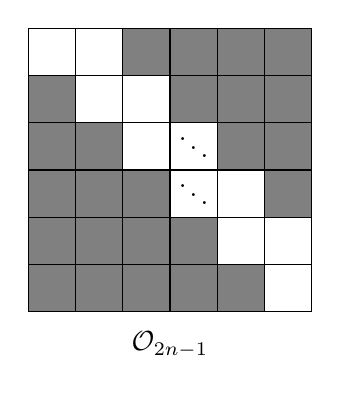
\begin{tikzpicture}[scale=0.6]
    \fill[gray] (1,0) rectangle (7,6);
    \foreach \i/\j in {1/5, 2/5, 2/4, 3/4, 3/3, 4/3, 4/2, 5/2, 5/1, 6/1, 6/0} { \fill[white] (\i, \j) rectangle (\i + 1, \j + 1); }
    \node at (4.5,3.65) {$\ddots$};
    \node at (4.5,2.65) {$\ddots$};
    \draw (1,0) grid (7,6);
    \path (1,-1.5) rectangle (7,6);
    \node at (4, -0.7) {$\mathcal{O}_{2n-1}$};
  \end{tikzpicture}
  ~
  \begin{tikzpicture}[scale=0.6]
    \fill[gray] (1,0) rectangle (7,6);
    \foreach \i/\j in {1/5, 1/4, 2/4, 2/3, 3/2, 3/3, 4/1, 4/2, 5/1, 5/0, 6/0} { \fill[white] (\i, \j) rectangle (\i + 1, \j + 1); }
    \node at (3.5,2.65) {$\ddots$};
    \node at (4.5,2.65) {$\ddots$};
    \draw (1,0) grid (7,6);
    \path (1,-1.5) rectangle (7,6);
    \node at (4, -0.7) {$\mathcal{O}_{2n-1}^\intercal$};
  \end{tikzpicture}
  ~
  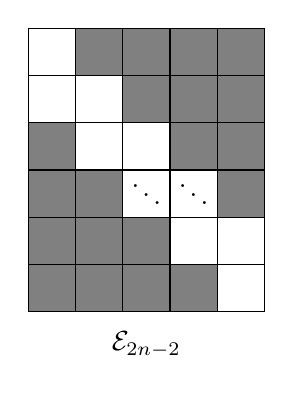
\begin{tikzpicture}[scale=0.6]
    \fill[gray] (1,0) rectangle (6,6);
    \foreach \i/\j in {1/4, 1/5, 2/3, 2/4, 3/2, 3/3, 4/1, 4/2, 5/0, 5/1} { \fill[white] (\i, \j) rectangle (\i + 1, \j + 1); }
    \node at (3.5,2.65) {$\ddots$};
    \node at (4.5,2.65) {$\ddots$};
    \draw (1,0) grid (6,6);
    \path (1,-1.5) rectangle (6,6);
    \node at (3.5, -0.7) {$\mathcal{E}_{2n-2}$};
  \end{tikzpicture}
  ~
  \begin{tikzpicture}[scale=0.6]
    \fill[gray] (1,1) rectangle (7,6);
    \foreach \i/\j in {1/5, 2/5, 2/4, 3/4, 3/3, 4/3, 4/2, 5/2, 5/1, 6/1} { \fill[white] (\i, \j) rectangle (\i + 1, \j + 1); }
    \node at (4.5,3.65) {$\ddots$};
    \node at (4.5,2.65) {$\ddots$};
    \path (1,-0.5) rectangle (7,7);
    \draw (1,1) grid (7,6);
    \node at (4, 0.3) {$\mathcal{E}_{2n-2}^\intercal$};
  \end{tikzpicture}
  \caption[Block shapes for a m\'enage permutation.]{
    Examples of each of the four staircase-shaped boards.
    The first two boards are on grids of size $n \times n$,
    the third is on a grid of size $n \times (n-1)$ and the
    fourth is on a grid of size $(n-1) \times n$.
  }
  \label{fig:blockShape}
\end{figure}
